\documentclass{standalone}
\usepackage{xcolor,amsmath,amssymb,amsfonts}
\usepackage{fontspec}
\usepackage[T1]{fontenc}
\usepackage[tt=false, type1=true]{libertine}
\usepackage[libertine]{newtxmath}

\usepackage{tikz}
\usetikzlibrary{arrows.meta}
\definecolor{red}{HTML}{c63a44}
\begin{document}

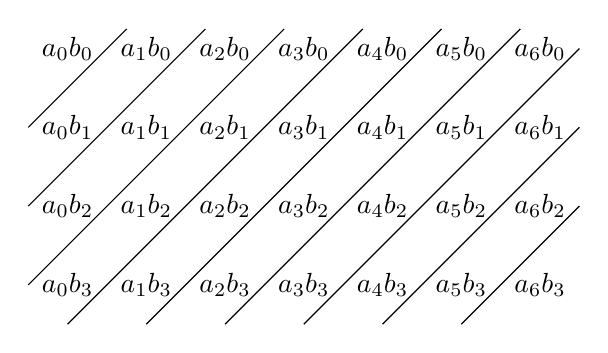
\begin{tikzpicture}
    \foreach\i in{0,...,6}{
        \foreach\j in{0,...,3}{
            \node at(\i,-\j)(\i\j){$a_{\i}b_{\j}$};
        }
    }
    \foreach\k in{0,...,8}{
        \pgfmathsetmacro\px{max(-0.5, \k - 3)};
        \pgfmathsetmacro\py{\px - \k - 0.5};
        \pgfmathsetmacro\qy{max(-0.25, \k - 6)};
        \pgfmathsetmacro\qx{\k - \qy + 0.5};
        \draw(\px,\py) -- (\qx,-\qy);
    }
\end{tikzpicture}

\end{document}